\documentclass[crop,tikz]{standalone}% 'crop' is the default for v1.0, before it was 'preview'
%\usetikzlibrary{...}% tikz package already loaded by 'tikz' option
\begin{document}
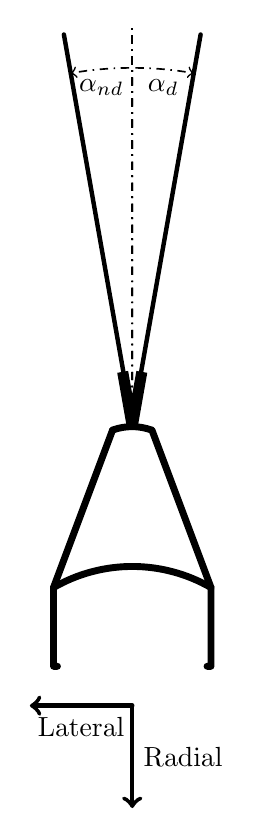
\begin{tikzpicture} [line width = 2.5 pt]
% rim
\draw[line cap = round, line join = round] (0.05,0)--(0,0) --(0,1) -- (0.75,3) ;
\draw[line cap = round, line join = round] (0.75,3) arc [start angle = 110, end angle = 70, radius = 0.725];
\draw[ line cap = round, line join = round] (1.25,3) -- (2,1) --(2,0)--(1.95,0);
\draw [line cap = round, line join = round] (0,1) arc [start angle = 120, end angle = 60, radius = 2];
% spokes 
\draw[ ultra thick, line cap = round, line join = round] (1,3.1) -- +(80:5cm);
\draw  [line width = 4 pt](1,3.05) -- +(80:0.7cm);
\draw[ ultra thick, line cap = round, line join = round] (1,3.1) -- +(100:5);
\draw [line width = 4 pt] (1,3.05) -- +(100:0.7cm);
\draw[semithick, dash dot] (1,3.1)  -- +(0,5);
\draw[semithick, dash dot,->] (1,3.1)  -- +(0,4.5) arc [start angle = 90, end angle = 100, radius = 4.5] node[midway, below] {$\alpha_{nd}$};
\draw[semithick, dash dot,->] (1,3.1)  -- +(0,4.5) arc [start angle = 90, end angle = 80, radius = 4.5] node[midway, below] {$\alpha_{{d}}$};
% axes
\draw[ultra thick, line cap = round,->]  (1,-0.5) -- +(-1.3,0) node[ midway, below] {Lateral} ;
\draw[ultra thick, line cap = round, ->]  (1,-0.5) -- +(0,-1.3) node[ midway, right] {Radial} ;
\end{tikzpicture}
\end{document}